\documentclass[a4paper, 12pt]{article}
\usepackage{listings}
\usepackage{color}
\usepackage[latin1]{inputenc}
\usepackage[T1]{fontenc}
\usepackage{graphicx}

\renewcommand{\lstlistingname}{Algorithm}% Listing -> Algorithm
\renewcommand{\lstlistlistingname}{List of \lstlistingname s}% List of Listings -> List of Algorithms

\lstset{
  morekeywords={*, path},
  language = Python,
  aboveskip = 2mm,
  belowskip = 2mm,
  showstringspaces = false,
  captionpos = b,
  columns = flexible,
  basicstyle = {\small\ttfamily},
  numbers = none,			% def = left
  numberstyle = \small\color{deepblue},
  breaklines = false,			%scelgo se troncare le righe o meno
  breakatwhitespace = true,
  tabsize = 3,
  emph = {True, False, return},          
  emphstyle=\color{deepblue},   
}

\begin{document}
\begin{center}
\LARGE\textbf{TVPR: Top View Person Re-identification}\\
\vspace{1em}
\small{Adel Massimo Ramadan, adel.massimo.ramadan@gmail.com\\
Riccardo Reali, finokkio@gmail.com\\
Ciolini Alberto, albeciolo@stud.unifi.it}\\
\vspace{0.75em}
X agosto 2017
\end{center}
\begin{center}
\end{center}

\tableofcontents
\lstlistoflistings

\newpage

\section{Introduzione}		%----------------------- Introduzione -------------------------------------------------------------------------------
Un importante compito per sistemi muti-camera distribuiti � il riconoscimento di un individuo in scene diverse, a tempi diversi: questo � noto come problema di \emph{Person Re-identification}.\\
La Person Re-identification � un'importante disciplina di settori come \emph{Human Computer Interaction},  \emph{Screen Monitoring}, \emph{Ambient Assisted Living} e molti altri rami di ricerca della \emph{Computer Vision}.
Si possono avere casi d'uso \emph{Online} o \emph{Offline}: nel primo caso l'analisi sul soggetto � immediata; mentre nel secondo caso si analizza la scena in differita (spesso avendo a disposizione una quantit� di informazioni maggiore).\\
Nella fattispecie del contesto studiato si parla di re-identification offline, basato su un sistema di \emph{depht cameras}\footnote{Asus Xtion Pro Live | \href{https://www.asus.com/3D-Sensor}}: le osservazioni di questo sistema vanno a comporre il dataset \emph{TVPR}\footnote{Universit� Politecnica delle Marche: \href{http://vrai.dii.univpm.it/re-id-dataset}}. In questo dataset sono presenti 23 video, ognuno nel formato 640x480, a un frame rate prossimo a 30fps, e disponibile in formato non compresso (\emph{.ONI}); in questi video compaiono 100 persone nel loro normale modo di fare quotidiano.
\begin{figure}
\centering
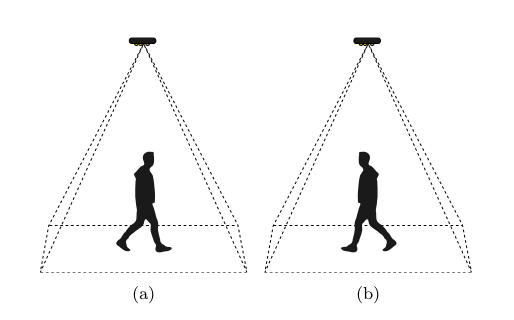
\includegraphics[scale=0.75]{immagini/base-scheme.png}
\caption{Mockup di un possiblie contesto: la camera, in alto, riprende la scena. La stessa persona passa nella scena (a) e nella (b).}
\end{figure}

\section{Obiettivi}        %----------------------- Obiettivi -------------------------------------------------------------------------------
Il principale obiettivo di questo progetto consiste nella realizzazione di un sistema in grado di stabilire se, dato un soggetto osservato al tempo $t_{0}$, questo sia presente o meno in un altra osservazione effettuata al tempo $t_{1}$. Il sistema dovr� essere in grado di effettuare questi confronti avvalendosi unicamente delle immagini di profondit�, si tratta quindi di un argomento ancora poco studiato dato che numerosi studi condotti sin'ora si sono avvalsi anche del dato relativo ai frame a colori.\\
Diventa quindi obiettivo anche il creare una buona base di partenza per un problema del genere, ed a prescindere dai risultati sar� un traguardo anche una consistente e strutturata analisi preliminare del problema.\\
La metrica per determinare la similarit� tra due persone sar� scelta a piacere tra \emph{3D - Shape Context\footnote{--riferimento}} e  \emph{3D - Shape Context\footnote{--riferimento}}. 
\newpage

\section{Analisi}        %----------------------- Analisi -------------------------------------------------------------------------------
In questa sezione il tema affrontato sar� la trattazione dei dati a disposizione: l'elaborazione di questi e la definizione dei modelli a cui sar� applicata la strategia risolutiva.\\
In virt� di sistema offline � possibile un ampia manipolazione dei dati, in modo tale da renderli pi� facili da analizzare: infatti in contesti online la velocit� dell'algoritmo � un elemento cruciale e non vi � il tempo materiale per applicare delle semplificazioni importanti.

\subsection{OpenNI file reader} %----------------------- ONI ----------------------------
\begin{figure}
\centering
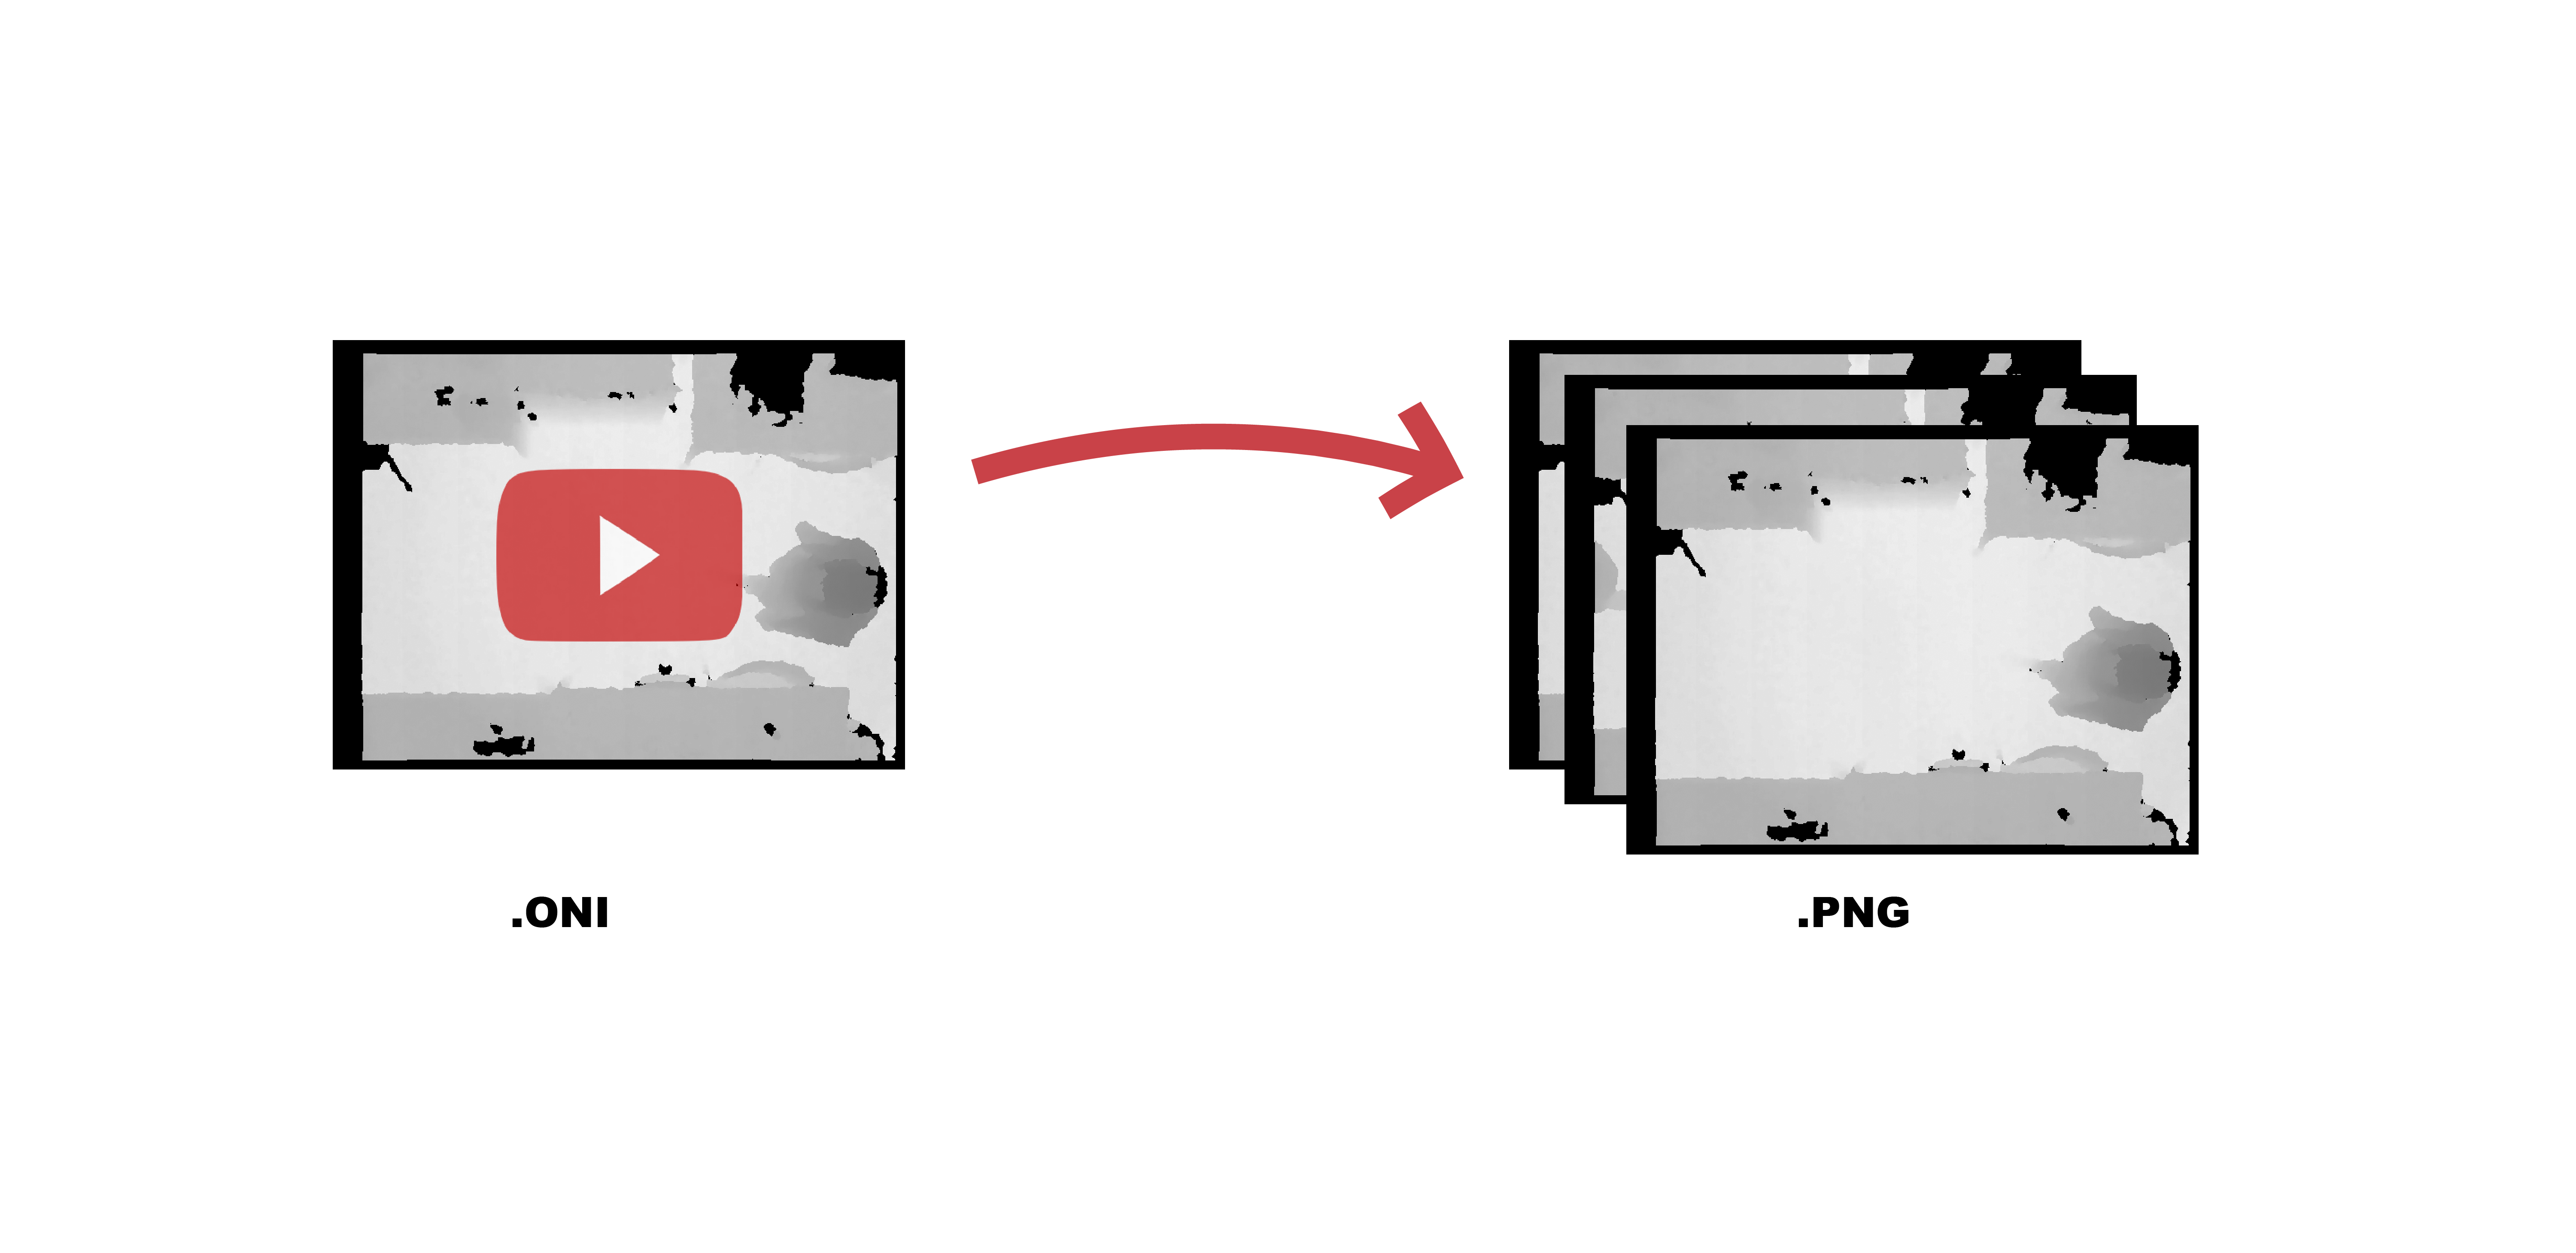
\includegraphics[scale=0.1]{immagini/img-02.png}
\end{figure}

Il dataset a disposizione comprende, come gi� introdotto, 23 filmati: ognuno di questi � presente sia in formato \emph{.avi} che in formato \emph{.oni}. Il primo come sappiamo comporta una compressione di tipo lossy, mentre il secondo � un tipo di dato raw, quindi diventa preferibile lavorare con quest'ultimo per non subire perdite di informazioni dovute alla compressione.\\
Questo formato conserva informazioni relative al frame di profondit� (depth frame), RGB e IR (InfraRed frame). Il dato che risulta di specifico interesse per il nostro scopo � quello relativo alla profondit�.
Per leggere questo formato sono disponibili delle API disponibili su \emph{Structure.io\footnote{\href{https://structure.io/openni}}}.
Grazie a queste � possibile scrivere il codice, riportato in \lstlistingname \ref{oniReader} che consente la lettura dei frame di profondit� dal dataset e la scrittura di questi come PNG.

\lstinputlisting[caption = Oni to PNG converter, label = oniReader]{codes/readerONI-sample.py}

\\� importante sottolineare che i depth frame sono codificati in scala di grigi a 16 bit, ma nonostante ci� il range effettivo dei colori � circa 7-3500. Non si usano perci� 16 bit effettivi (ne basterebbero 12): questo � dovuto al fatto che il sensore utilizza 1 livello per ogni millimetro, ed essendo il campo raggiungibile tra 7mm e 3,5m ne segue che la banda utilizzata sia molto ridotta.\\
 \emph{Es: un punto a 2 metri dal sensore sar� rappresentato con il valore 2000}.
 
 
\subsection{Clasificare le Persone} %----------------------- Classify ----------------------------
Per quanto riguarda la classificazione delle persone, la strategia adottata � piuttosto semplice
\lstinputlisting[caption = Oni to PNG converter, label = oniReader]{codes/classifyPerson-sample.m}

\subsection{Central Frame Detection} %----------------------- Central ----------------------------
\lstinputlisting[caption = Oni to PNG converter, label = oniReader]{codes/centralFrameDetector-sample.m}

\subsection{Normalizzare le Persone} %----------------------- Normalize ----------------------------
\lstinputlisting[caption = Oni to PNG converter, label = oniReader]{codes/normalizePerson-sample.m}

\end{document}